\documentclass{article}
\usepackage{graphicx}
\usepackage{listings}
\usepackage{textcomp}
\usepackage{array}
\usepackage{bold-extra}
\usepackage{enumitem}
\usepackage{hyperref}
\usepackage{amsfonts}
\usepackage{mathtools}
\usepackage{subcaption}

\usepackage[superscript,biblabel]{cite}

\DeclarePairedDelimiter{\set}{\{}{\}}

\DeclarePairedDelimiter{\abs}{\lvert}{\rvert}

\hypersetup{
    colorlinks=true,
    linkcolor=blue,
    filecolor=magenta,      
    urlcolor=cyan,
}

\urlstyle{same}

\newcolumntype{x}[1]{>{\centering\arraybackslash\hspace{0pt}}m{#1}}

\title{Sorting arrays using $k$-way comparisons}
\author{Emil Indzhev}

\begin{document}

\maketitle

\section{Introduction}

Sorting an array using a 2-way comparison function is a well studied problem in Computer Science. We generalize the problem to use a $k$-way comparison function and modify existing algorithms to support that. Our focus is on minimizing the number of comparisons for a wide range of values of $k$, while also keeping the actual running time of the algorithms small. All algorithms and optimizations have been implemented and tested using a tasting framework designed for the problem.

Note, this essay is adapted from the statement and analysis of a competitive programming problem for selection of the Bulgarian national team for the IOI. All solution and testing framework implementations may be found at: \\
\url{https://github.com/indjev99/Competitive-Programming-Problems/tree/master/multisort}

\section{Problem statement}

\subsection{Mathematical formulation}

We need to sort a uniform random permutation $ P $ of $ n $ different elements. The permutation is hidden from us, but we can make $k$-way comparisons on it using the indices of the elements we want to compare. The answer to the query is a sequence containing the same indices as the query but ordered in increasing order with respect ot the indexed elements of $ P $. More formally, for a query $ I $ we get the answer $ J $ where:

$$ I \subseteq \mathbb{Z}_n : \abs{I} \leq k $$

$$ (J_t)_{t=0}^{\abs{I} - 1}  : \set{J_t}_{t=0}^{\abs{I} - 1} = I \land \forall s,t \in \mathbb{Z}_{\abs{I}} \cdot s < t \rightarrow P_{J_s} < P_{J_t} $$

Our goal is to find a sequence $ R $ of $ n $ indices ordered in increasing order with respect ot the indexed elements of $ P $. We want to do this with as few queries as possible, while also being fast in terms of actual run time. Formally:

$$ (R_t)_{t=0}^{n - 1}  : \set{R_t}_{t=0}^{n - 1} = \mathbb{Z}_n \land \forall s,t \in \mathbb{Z}_n \cdot s < t \rightarrow P_{R_s} < P_{R_t} $$

\subsection{Testing framework}

To simplify things we present our testing API.

Our algorithm is given $ n $ and $ k $ and should return $ R $ as a \verb|vector|. It is called with the function:

\begin{lstlisting}
std::vector<int> multisort(int n, int k);
\end{lstlisting}

It can use the compare function by passing $ I $ as a \verb|vector| of indices and getting $ J $ back as the same \verb|vector|, which is reordered in-place:

\begin{lstlisting}
void compare(std::vector<int>& elems);
\end{lstlisting}

At the end the testing framework verifies that $ R $ is correctly sorted and prints the number of comparisons used. It can also perform many runs and average them or take their maximum. This is used for more detailed analysis of the performance of our solutions.

\section{Theoretical lower bound}

One way to get a lower bound on the number of comparisons needed is to analyze the amount of information we need to find and divide it by the maximum amount of information we can get per comparison. The amount of inforation $ \mathrm{H}(X) $ (in natural units of information) in a discrete random variable $ X $ that can take values in $ V $ according to some probability distribution $ \mathbb{P} $ is \cite{informationtheory}:

$$ \mathrm{H}(X) = - \sum_{v \in V} \mathbb{P}(X = v) \ln{\mathbb{P}(X = v)} $$

This is maximized when $ X $ is uniformly distributed \cite{informationtheory} and then:

$$ \mathrm{H}(X) = - \abs{V} \frac{1}{\abs{V}} \ln{\frac{1}{\abs{V}}} = \ln{\abs{V}} $$

Therefore, the amount of information in $ P $ is $ \ln{n!} $ and the maximum possible amount of information in a query is $ \ln{k!} $. We then get the following lower bound for the number of queries needed, which we simplify using Stirling's approximation:

$$ \mathrm{Q}(n, k) = \frac{\ln{n!}}{\ln{k!}} = \frac{ n \ln{n} - n + \mathrm{O}(\ln{n}) }{ k \ln{k} - k + \mathrm{O}(\ln{k}) } \approx \frac{n}{k}\log_k{n} $$

Note, that later when we are numerically comparing the performances of various algorithms to the theoretical lower bound we will use a much more exact value of $ \mathrm{Q}(n, k) $, obtained by expanding the $ \mathrm{O}(\ln{n}) $ and $ \mathrm{O}(\ln{k}) $ terms.

\section{Scoring system}

To be able to easily compare different algorithms we will reference the scoring system that was used at the competition. It runs the algorithm on $ T = 30 $ of tests with fixed $ n = 20000 $ and varying $ k $ where $ 2 \leq k \leq 1000 $ with a roughly logarithmic distribution. Finally,  for each of $ T $ tests the solution gets a score of:

$$ \frac{100}{T} \times \min\left(1, \left(\frac{bestScore + 1}{solutionScore + 1}\right)^{0.75}\right) $$

Here $ solutionScore $ is the number of comparisons used by the algorithm in this instance and $ bestScore $ is the number of comparisons used by the best found algorithm in the worst out of $ T $ runs (on tests with the same $ n $ and $ k $). This is done to reduce the variance of $ bestScore $ and to guarantee that the best solution can get the maximum score with a significant probability for any seed.

We use this score metric to get a rough idea of how good various algorithm are. We will present a more detailed breakdown of the performances of our best algorithms.

\section{Dummy algorithm}

One dummy algorithm we can use as a benchmark is to only use 2-way comparisons, e.g. by calling \verb|std::sort| with a custom comparison function which uses \verb|compare|. This needs about $ \log_2{n} $ comparisons and receives 10 points.

\section{Quicksort}

The first main approach we examine is one based on quicksort \cite{quicksort}. Of course, a plain quicksort is essentially the same as \verb|std::sort|, but it allows us to freely modify it.

\subsection{Bottom}

The easiest thing to change is to add a new base case to the recursion: when $ 2 \leq n \leq k $ we sort the entire remaining array with one query. This solution gets 11 points. We call this optimization ``bottom" as it happens on the bottom layers of the recursion. For any other optimization we present, we will always use this one together with it.

\subsection{Multibranch}

One way to use the $k$-way comparison on each iteration of the recursion is to divide the array into $k$ parts (instead of only 2) - we call this ``multibranch". We do this by choosing $ k - 1 $ random pivots, and then we compare each element with the pivots. After that we look where in the list the new element is (it is best to do this using binary search); the element belongs to the same part as its position in this ordered list.

This uses about $ n $ queries per level of the recursion and in the best case (with even splits between the pivots) it has $ \log_k{n} $ levels. In the average case we still have $ \mathrm{\Theta}\left( \log_k {n} \right) $ levels as long as $ n \gg k $. In total, we get about $ \mathrm{\Theta}\left( n \log_k{n} \right) $ comparisons, which is not too good. Also, the constant factor is big due to the splits not being that equal. This gets 21 points.

\subsection{Multiway}

Another much better simple idea is to divide into 2 parts as usual, but process $ k - 1 $ elements at a time. We fix a random pivot and compare the rest of the elements in batches of $ k - 1 $ against it. We sort them into the two parts as usual (this can easily be done in linear time per batch).

This behaves exactly like regular quicksort, but uses about $ k $ times fewer comparisons. Therefore, it needs $ \mathrm{\Theta}\left( \frac{n}{k} \ln{n} \right) $ queries, which is much better than before. This solution receives 53 points.

\subsection{Smart pivot}

It is well-known using a few comparisons to get a better pivot is usually worth it. However, since we focus on values $ k > 2 $, we can do even better by using 0 additional comparisons. We fix the pivot only after the result of the first query, we use its median element. Note that it is important to pick the elements for the first query randomly from the whole array, so that it is representative of the array. This helps the pivot to be a better approximation for the median, which significantly reduces the number of comparisons needed. This receives 65 points.

\subsection{Multiway multibranch}

The ``multibranch" optimization reduces the number of queries by a factor of $ \ln{k} $ and the ``multway" one -- by a factor of $ k $. It is a good idea to combine them to achieve the wanted complexity. Naively, we can try having $ \frac{k}{2} $ pivots and process elements in batches of $ \frac{k}{2} $, but after a bit of thinking (and calculating or trying) this is clearly not optimal. Let us call the number of pivots $ s $. Then, the optimal value of $ s $ that we can calculate using a few simplifications is the one that maximizes $ (k - s) \ln{(s)} $. That value is $ s = \frac{k}{ \mathrm{W}(ke) } $.

However, these simplifications turn out to be too great. In practice the splits are not perfect, $ n $ also matters due to not fully utilized queries and both of these concerns propagate up the recursion. Given that $ n = 20000 $ is fixed (for our testing), it is better to use some constant for $ s $  (such as $ s = 4 $) and only tweak it for small $ k $.

This solution gets 74 points with random pivots and 80 points using the ``smart pivots" optimization (we use $ s $ equally spaced elements from our first query for the pivots). With some more non-intuitive tweaking of $ s $ (and ``smart pivots") we can get 87 points, still using a fixed $ s $ that depends only on $ k $.

\subsection{Dynamic programming}

To automatically determine a good value for $ s $ we can use the dynamic programming approach. Here, $ s $ will also depend on the current $ n $ and thus will potentially be different at each call of the recursive sort function. Since $ k $ is fixed for the whole run and $ n $ varies, it makes sense to have a 1-dimensional array indexed by $ n $. It will contain the optimal number of pivots to use for the current $ n $. To that end, in another array we calculate the expected number of queries to sort an array with $ n $ elements given that we use the optimal values of $ s $. Then, to calculate the next values for the two arrays, we try every possible (reasonable) value of $ s $, calculate the expected number of comparisons needed using it for the current iteration. Finally, in the first array we store the $ s $ that minimized that quantity and in the second array -- the minimal quantity itself.

The expected number of queries needed to sort an array of length $ n $ is the number of queries needed to split its elements into $ s + 1 $ parts plus the expected number of queries to sort each of those parts. To partition its elements we need $ \frac{n - s}{k - s} $ comparisons. For now, we can assume that the $ s + 1 $ parts will be all equal, so we would need $ (s + 1) \times dp\left[ \frac{n - s}{s + 1} \right] $ queries to sort them. In fact, instead of rounding the lengths of the parts up or down (effectively creating or removing elements) it is better to have some number of them rounded up and some rounded down, so that their sum is $ n - s $.

Note, to improve run time when trying to find the best value of $ s $ for some $ n $ we only look at values close the optimal $ s $ for $ n - 1 $, since it makes sense to assume they would be close. We also cap it at $ \frac{k}{2} $, since anything above that is clearly not optimal. The time for the precompute is $ \mathrm{\Theta}\left( n \right) $. There is no $ k $ factor due to the optimization described here.

This still ignores the random partitioning and thus it underestimates the expected number of queries needed. However, it is relatively consistent with that underestimation and its predicted optimal values for $ s $ are quite good. In the end, this finally achieves the optimal complexity and gets 95 points, though remember on each test the solution is compared to the worst run of the best solution (not its average).

\subsection{Monte Carlo DP}

It would be best to use the full distribution for all possible partitions and do the DP that way. However, that is not easy to calculate and more importantly would take at least $ n^2 $ time. So, we satisfy ourselves with a Monte Carlo approach, i.e. use randomization. For now, for each $ n $ we generate a single random sample of $ k $ different numbers in $ \mathbb{Z}_n $ in increasing order -- that is our initial query.

We can do this in $ \mathrm{\Theta}\left( k \ln{k} \right) $ time using a set, or with some clever tricks using just a ``used" array (that holds timestamps, so we don't need to clear the array each time) and a vector, which we sort at the end. The second one has a better constant, but is still not great. We can also use a counting sort approach (again with timestamps) in $ \mathrm{\Theta}\left( n + k \right) $ time, which is better in pracitce, especially for large $ k $. Then, for each value of $ s $ that we try, we calculate the expected number of queries conditioned on the sample in $ \mathrm{\Theta}\left( s \right) $ time.

The total run time of the precompute is $ \mathrm{\Theta}\left( n^2 + nk \right) $, which is not practical due to the $ n^2 $ factor. However, in terms of comparisons this is very close to the best found solution and gets almost 100 points.

\subsection{Running sample}

The slowest step in our previous algorithm was the sample generation. A way to fix this is to keep one running random sample. Then, for each $ n $ we update the sample by including $ n $ with a probability of $ \frac{k}{n} $ in which case we remove a random old element from the sample.

This still keeps any individual sample uniform, but the samples at different $n$-s are no longer independent, which slightly worsens the performance of the algorithm. We can fix this by taking advantage of the fact that generating a sample is now much faster by keeping many independent running samples (we use a fixed number of 10).

This solution is still faster and also better than our previous one. Its precompute runs in $ \mathrm{\Theta}\left( nk \right) $ time and it is our best solution with 100 points.

\section{Merge sort}

Another general approach we can try is one based on merge sort \cite{mergesort}. A standard merge sort gets 12 points, since it performs fewer comparisons than quicksort. Of course, it is again a good idea to use the ``bottom" optimization. In general, most of the optimizations we discussed for quicksort would apply for merge sort too.

\subsection{Multibranch}

Here we have an analogous optimzation to the one for quicksort. We split the array into $k$ equal chunks and recursively sort each of them. Then, at each merge step, we compare the first elements from each chunk. Finally, we take out the minimum of those and add it to the result (and increment the pointer for the chunk it came from).

The implementation requires tracking $k$ pointers and also where each element came from, but that is not too difficult. In fact, with a bit of ingenuity we can achieve $ \mathrm{\Theta}\left( n \ln{n} \right) $ time. The trick is, when we remove the minimum element, to directly replace it with the next elements from the chunk it came from. Thus, each merge step is $  \mathrm{\Theta}\left( 1 \right) $  time.

As before, the ``multibranch" optimization reduces the number of queries used by a factor of $ \ln{k} $, for a total of $ \mathrm{\Theta}\left( n \log_k{n} \right) $ queries. This solution gets about 21 points.

\subsection{Multiway}

The way ``multiway" works in merge sort is similar to before. We simply process the elements in batches. This is done when merging. We take $ \frac{k}{2} $ elements from each of the two chunks we need to merge. After we compare them against each other, we can be sure that a certain prefix of theirs should be the next thing we add to the merged array. That prefix is all elements except the maximal suffix of elements coming from the same chunk.

We exemplify this by writing `A' for elements coming from the first chunk and `B' for ones from the second chunk. Suppose that the result of one query is: ABBABBAA. The prefix we can add to the merged array is ABBABB, and we aren't sure about the final AA. This is because the next B, which we haven't compared against these elements, could come before the As, between them or after them.

Since the two chunk that we need to merge are of equal size and contain randomly picked elements, they grow at about the same rate. Therefore, there shouldn't be a bias towards either part when merging and thus we should be able to utilize our queries almost fully. Even in the worst case (all elements from one half being before all elements from the other one), we still process $ \frac{k}{2} $ elements per comparison. Therefore, this solution uses $ \mathrm{\Theta}\left( \frac{n}{k} \ln{n} \right) $ queries. As a result, it gets 62 points.

\subsection{Alignment}

Since we have more control over how we split the array in merge sort than in quicksort, it is a good idea to orchestrate the splits to get full use of our bottom level comparisons, i.e. Split the array in chunks of size $ k $ and then merge them (in the usual balanced way). It is simplest to implement this directly in the recursion by rounding the point where we split to the nearest multiple of $k$. This ensures that all but the rightmost bottom level calls of the recursion will have an array of size exactly $k$. This receives 65 points.

\subsection{Multiway multibranch}

Again, we can combine these two optimizations produce a better solution. First, we split the array into $ s $ eual chunks and recursively sort them. Then, at each merge step, we compare the first $ \frac{k}{s} $ elements from each chunk. After that, we take out a prefix of that sorted subarray, according to analogous rules to the one for ``multiway" (we stop as soon as we have taken all elements from any one chunk). Again, we need to keep track of various pointers, counters, etc., as described above. 

Note that in the worst case we only extract $ \frac{k}{s} $ elements per merge step. However, the average case is closer to $ k $, especially when $ s $ is small, since the elements are uniformly distributed among the chunks. This can be formalized using a more careful analysis.

Therefore, if $ s $ is chosen well, this solution will have the optimal query complexity. Furthermore, it does $ \mathrm{\Theta}\left( k \right) $ per query. Thus, its total run time is $ \mathrm{\Theta}\left( n \log_k{n} \right) $, which makes it more than feasable.

So, we just need to choose $ s $. As with quicksort, we can just hardcode simple rules for using $ s $ up to $ 5 $ and receive 74 points. Alternatively, we can run tests for more values of $ k $, in order to have more complicated rules for $ s $, as well as make more minor improvements to the merging and receive 86 points. As expected, this is very close to the results the quicksort solution gets.

\subsection{Further development}

More complex strategies for chosing $ s $ at each step, depending on both $ n $ and $ k $, have not been explored. A DP approach (perhaps with random sampling), similar to the one for quicksort, will likely perform well and receive close to 100 points.

Another possible improvement, is to add a version of the ``alignment'' optimaztion to the above merge sort solution.

\section{Topological sort}

The last approach we have examined is topological sort, more specifically Kahn's algorithm \cite{topsort}. Elements correspond to vertices and the results of queries -- to directed edges between the sequential elements in the result of the query (from the smaller element's vertex to the larger one's vertex). This records all information that we have gotten and therefore, if it somehow happens that we have made enough comparisons, we can simply run topological sort on the constructed graph to get the answer.

We can try making a lot of random queries and then running topological sort, but this is clearly not ideal. For one, it is possible that there is no unique topological sorting after our queries, in which case we need to continue making more of them. However, this directs us to a good way to make queries.

At each iteration, we start performing topological sort. If at some point there is ambiguity on which element to pick next (i.e. there is more than one element in the queue), we know that we haven't made enough queries to get the answer. Then, we start putting all the elements that we pop from the queue (in the main loop of the topological sort) in the comparison set. When that set reaches $ k $ elements (or the topological sort is done), we break from that loop, compare all the elements in the set and add edges in the graph as described before. Finally, we repeat the whole process again until we get unambiguous topological sorting, which must be the answer.

Note, it is tempting (and perhaps more intuitive) to compare only the elements among which the next one might be, i.e. when we detect an ambiguity because there is more than one element in the queue, we break immediately and compare only those elements. This would work too, but does not take full advantage of our queries. Therefore, what we described is better; its comparison set is a superset of this more minimal one and thus gets us more information, which might be useful.

For the implementation it is convenient to determine the first element (the minimum) before the main part of the algorithm. The alternative is to add a dummy source node with an edge to each of the other nodes, but this is less convenient as we then need to take care not to include it in our answer.

The big problem here is the run time. Each iteration takes $ \mathrm{\Theta}\left( \frac{n}{k} \ln{n} \right) $ times, but we do one full iteration per query we make. Even if this is optimal in terms of number of queries, i.e. it makes $ \mathrm{\Theta}\left( \frac{n}{k} \log_k{n} \right) $ queries, it will take $ \mathrm{\Theta}\left( \frac{n^2}{k} \log_k{n} \right) $ time in total. This is actually feasible for relatively large $k$, but definitely not for small $k$. After testing, it runs in the time limit for the problem for $ k > 40 $. To get its score, we run the dummy solution (\verb|std::sort|) for $ k \le 40 $ and otherwise this solution. This receives 67 points.

\subsection{Rollback}

In order to fix the problem described above, we need to notice that each iteration will do exactly the same up to the point where ambiguity is reached. Therefore, we can start each iteration at the point right before that. We implement this using a stack where we store all changes made on the state of the program at each step of the topological sort. Furthermore, at the start of each step, as long as we haven't reached ambiguity, we push a validness marker to the stack. When we reach ambiguity and start building up the comparison set, we stop pushing the validness marker to the stack. Then, after we perform the comparison, we backtrack using the stack. For each element that we pop, we reverse the changes to the state described by it. We do this until we reach a validness marker (which we leave in place). This way we restore the program to the state it had before it reached the ambiguity (though still keeping the new edges from the comparison).

Since each iteration does extra work only for the $k$ elements that it compares, we get $ \mathrm{\Theta}\left( k \right) $ time per iteration (and thus per comparison) plus $ \mathrm{\Theta}\left( n \right) $ overall for the actual valid/unambiguous topological sort (this can be formalized with an amortized analysis). Again, if we assume that this algorithm performs $ \mathrm{\Theta}\left( \frac{n}{k} \log_k{n} \right) $ comparisons, the total run time is $ \mathrm{\Theta}\left( n \log_k{n} \right) $, which is very good.

It turns out that the solution behaves essentially like it makes $ \mathrm{\Theta}\left( \frac{n}{k} \log_k{n} \right) $ queries for $ k > 2 $, but it behaves really badly for $ k = 2 $. This is not a big problem as we can just use the dummy solution in that case, where it is optimal anyway. This gets 97 points, which is almost as much as our quicksort solution with a much lower run time.

\subsection{Comparison complexity}

Intuitively, it makes sense that this will have the optimal query complexity, but we have no proof of this fact. It makes relatively good queries (in the sense that it is asking about relevant elements) and doesn't waste any of the information it gets. The queries are still not optimal as this whole algorithm is essentially a complicated selection sort; in order to proceed unambiguously, we need to find the minimal remaining element and put it at the end of the sorted array we are building, which is exactly what selection sort does. Our advantage comes from storing all the information we have gotten, but this still doesn't help us if we make really bad queries.

When trying to find this minimal remaining element, we can compare the current minimum found with all the other elements, which is the bad option that leads to quadratic behaviour since we end up with no extra information after we extract the minimum, or we can try to do it in balanced tree way, which leads to $ n \ln n $ behaviour since we can reuse almost all the information we got for the next step. After examining our solution it turns out that it is essentially using the first option since it is deterministic, and we always get the same order for the elements in the queue (and thus we always start with the same potential minimum). This is actually not a big problem for larger $ k $ since almost all the information we get is from comparing elements further down the chain for the topological sort (and not just trying to find the minimum). However, for $ k = 2 $ this leads to quadratic behaviour, as it is just doing plain selection sort.

\subsection{Further development}

A possible further development is to look into preventing this behaviour. One possible way might be to use some randomization in the order in which we process elements. Alternatively, we can try to actively prioritize elements that haven't been compared as many times (nodes with a lower degree in the graph). Both of those are non-trivial to implement due to our optimizations to keep the run time low.

\section{Algorithm comparison}

Let us first summarize the advantages and disadvantages of our best algorithms in each category.

Topological sort uses all the information that gets from the queries, but it is unable to make queries as well since it must always focus on finding the next smallest element.

Quicksort throws away a lot of the information that it gets since it doesn't care about the relative order of the elements in the same group (just which group they belong to); effectively it only distinguished about $ (k - s)^{(s + 1)} $ outcomes, as opposed to $ (k - s)! $ or even $ k! $. On the other hand, it is able to make really good queries considering the outcomes it cares about (close to uniform distribution among them due to the well chosen pivots).

Finally, merge sort is unable to make queries that can give a lot of information since it already knows the relative orders of the elements in the $ s $ chunks, so there are only $ \frac{k!}{ {(k / s)!}^s } $ possible outcomes. However, it is able to use almost all of that information and its queries are quite good in that setting. Its main problem is that it seems harder to find a good way to choose $ s $.

We can imagine a near optimal algorithm that greedily chooses the query that gives the most information by iterating over all possible queries and calculating the probabilities of each of their outcomes based on the answers to the previous queries. The problem is that this is not close to feasible in practice. However, it is possible that there exists an algorithm that combines the advantages of the ones we described and performs even better.

\section{Empirical performance}

Here we present the performance of our two best algorithms (based on quicksort and topological sort). We plot the number of queries used by both algorithms as a function of $ k $. To simplify the plot, we show the number of queries used relative to the theoretical minimum for that $ n $ and $ k $. As we can see in \ref{fig:performance}, our quicksort solution seems to make up to about 2 times the theoretical minimum for a wide range of values for $n$ and $k$. The topological sort solution also performs quite well, though not as well.

\section{Conclusion}

We examined a more general version of the well studied problem of sorting an array using comparisons. After trying approaches based on various standard algorithms, we develop two solutions with the optimal complexity in terms of number of comparisons (this is only conjectured for topological sort).

The best one, based on quicksort, uses about twice as many queries as the theoretical minimum and is feasible for moderate $ n $ and $ k $. However, the $ nk $ term in its run time prevents it from being practical for large $ n $ and $ k $ such as $ n = 10^6 $ and $ k = 1000 $, where a single run takes several seconds on a modern processor. Note, that this is due to the precompute step and not the actual sorting. So, this is not an issue, if we expect to be using the sort function many times with the same value of $ k $.

The other solution, based on topological sort, is harder to characterize as we have no proof of its complexity. However, it performs almost as good as the quicksort solution and runs in much lower time, which makes it feasible anywhere where a regular sorting algorithm would be feasible. It still has some problems for small $ k $, which might also affect its performance for any $ k $. Fixing those might lead to an even better overall solution.

\begin{figure}[h]
\centering

\begin{subfigure}{0.85\textwidth}
\centering
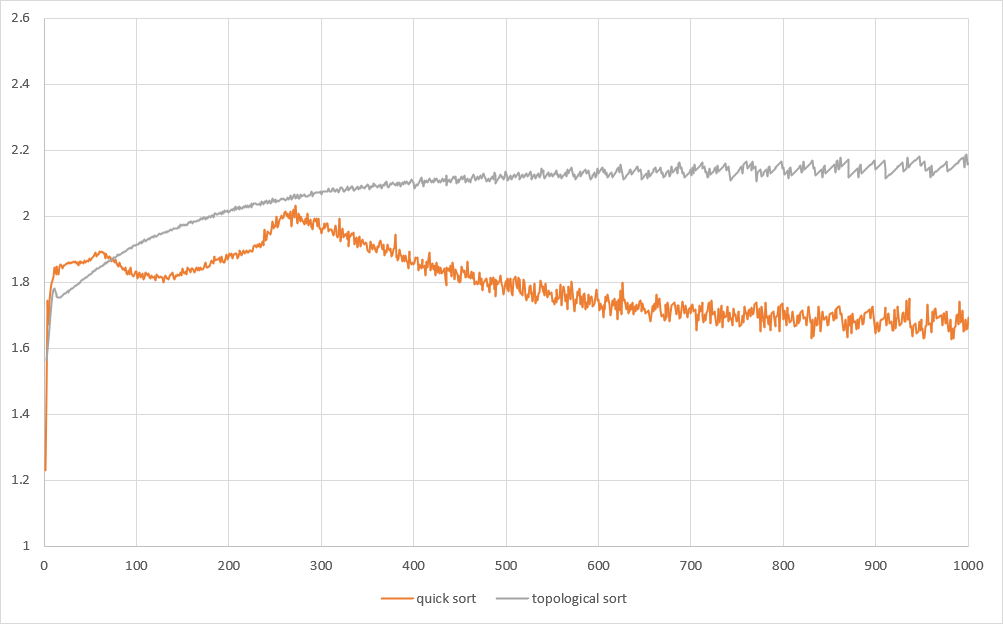
\includegraphics[width=\textwidth]{2e4}
\caption{$ n = 2 \times 10^4 $; mean of 20 runs for each $k$; $k$ is in increments of 1.}
\label{fig:2e5}
\end{subfigure}

\begin{subfigure}{0.85\textwidth}
\centering
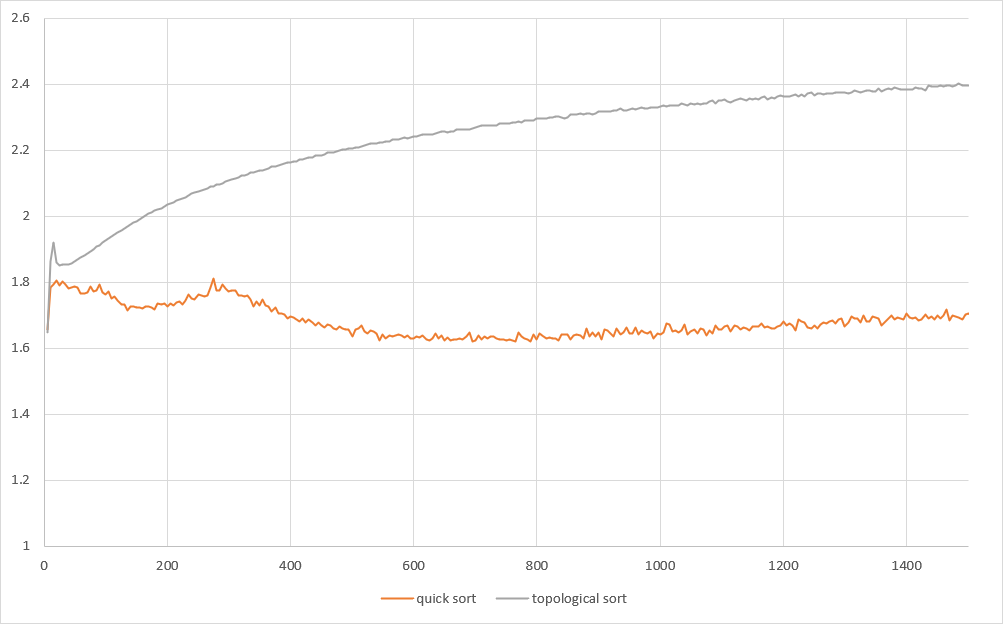
\includegraphics[width=\textwidth]{1e6}
\caption{$ n = 10^6 $; single run for each $k$; $k$ is in increments of 5.}
\label{fig:1e6}
\end{subfigure}

\caption{}
\label{fig:performance}

\end{figure}

\bibliographystyle{unsrt}
\bibliography{bibliography}

\end{document}